% Created 2019-07-29 Mon 16:45
% Intended LaTeX compiler: pdflatex
\documentclass[11pt]{article}
\usepackage[utf8]{inputenc}
\usepackage[T1]{fontenc}
\usepackage{graphicx}
\usepackage{grffile}
\usepackage{longtable}
\usepackage{wrapfig}
\usepackage{rotating}
\usepackage[normalem]{ulem}
\usepackage{amsmath}
\usepackage{textcomp}
\usepackage{amssymb}
\usepackage{capt-of}
\usepackage{hyperref}
\usepackage[newfloat]{minted}
\usepackage{caption}
\author{Yi Zhang, William R. Gillespie}
\date{\today}
\title{Stan/Torsten tutorial example: Parametric time-to-event model}
\hypersetup{
 pdfauthor={Yi Zhang, William R. Gillespie},
 pdftitle={Stan/Torsten tutorial example: Parametric time-to-event model},
 pdfkeywords={},
 pdfsubject={},
 pdfcreator={Emacs 25.3.1 (Org mode 9.1.3)}, 
 pdflang={English}}
\begin{document}

\maketitle
\section{Model}
\label{sec:org92df8be}
We analyze the time to the first grade 2+ peripheral neuropathy
(PN) event in patients treated with an antibody-drug conjugate (ADC) delivering monomethyl auristatin E
(MMAE). We will simulate and analyze data using a simplified version of the
model reported in \cite{lu_time--event_2017}.
\begin{itemize}
\item Fauxlatuzumab vedotin 1.2 mg/kg IV boluses q3w \(\times\) 6 does.
\item 19 patients with 6 right-censored (simulated data).
\item To keep things simpler, we use the simulated individual CL and V values, and only model PD part of the problem.
\end{itemize}
\begin{figure}[htbp]
\centering
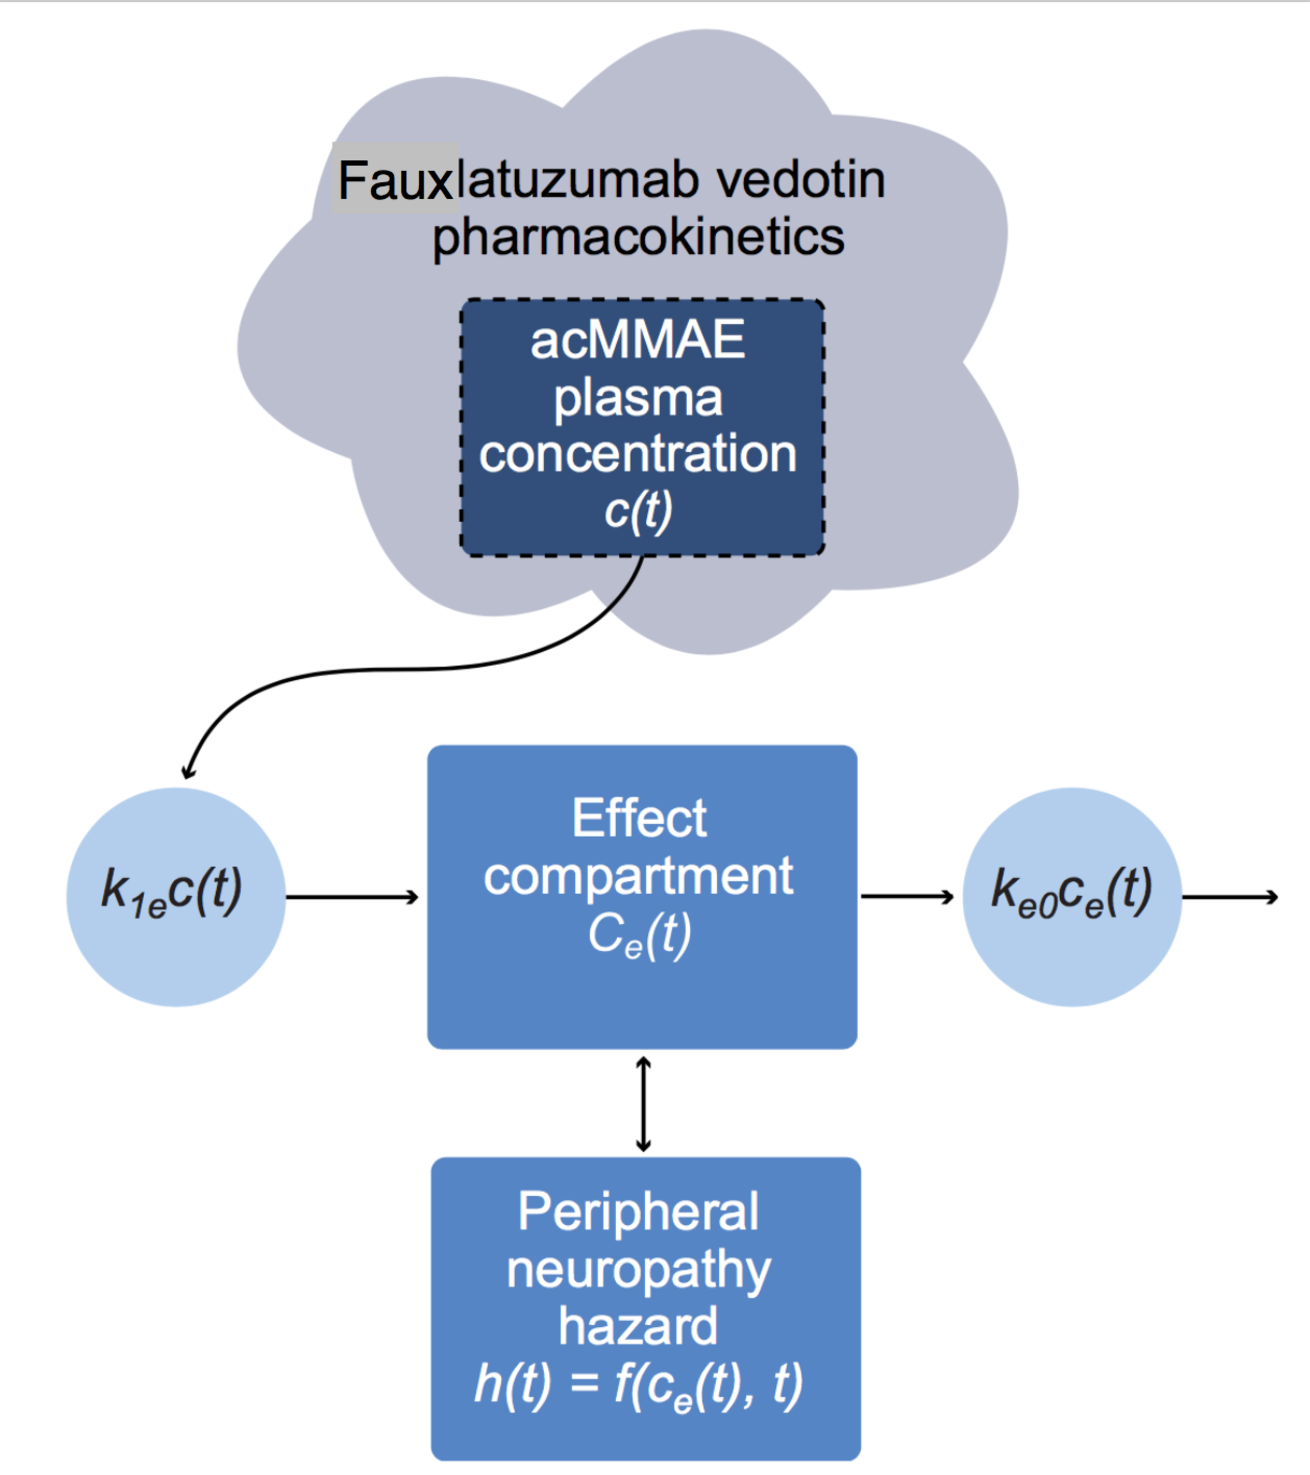
\includegraphics[width=0.4\columnwidth]{./lu2017Model.pdf}
\caption{Model scheme}
\end{figure}
\begin{itemize}
\item PN hazard is substantially delayed relative to PK exposure.
\item Hazard increases over time to an extent not completely described by PK.
\end{itemize}

Likelihood for time to first PN \(\ge\) 2 event in the \(i^{th}\) patient:
\begin{align*}
\lefteqn{L\left(\theta | t_{\text{PN},i}, \text{censor}_i, X_i\right)} \\
  &= \left\{ \begin{array}{ll}
     h_i\left(t_{\text{PN},i} | \theta, X_i\right) e^{-\int_0^{t_{\text{PN},i}} h_i\left(u | \theta, X_i\right) du}, &
    \text{censor}_i = 0 \\
     e^{-\int_0^{t_{\text{PN},i}} h_i\left(u | \theta, X_i\right) du}, &
     \text{censor}_i = 1
\end{array} \right.
\end{align*}
where
 \begin{align*}
   t_{\text{PN}} &\equiv \text{time to first PN $\ge$ 2 or right
     censoring event} \\
 \theta &\equiv \text{model parameters} \\
 X &\equiv \text{independent variables / covariates} \\
 \text{censor} &\equiv \left\{ \begin{array}{ll}
     1, & \text{PN $\ge$ 2 event is right censored} \\
     0, & \text{PN $\ge$ 2 event is observed} 
 \end{array} \right.
\end{align*}
One can see the expression
\begin{equation*}
  e^{-\int_0^{t_{\text{PN},i}} h_i\left(u | \theta, X_i\right) du}
\end{equation*}
as the survival function at time \(t\).

\begin{itemize}
\item Hazard of PN grade 2+ based on the Weibull distribution,
with drug effect proportional to effect site concentration of MMAE:
\end{itemize}
\begin{align*}
  h_j(t) &= \beta E_{\text{drug}j}(t)^\beta t^{(\beta - 1)} \\
  E_{\text{drug}j}(t) &= \alpha c_{ej}(t) \\
  c^\prime_{ej}(t) &= k_{e0} \left(c_j(t) - c_{ej}(t)\right).
\end{align*}

Overall ODE system including integration of the hazard function:
\begin{align*}
  x_1^\prime &= -\frac{CL}{V} x_1 \\
  x_2^\prime &= k_{e0} \left(\frac{x_1}{V} - x_2\right) \\
  x_3^\prime &= h(t)
  \end{align*}
where \(x_2(t) = c_e(t)\) and \(x_3(t) = \int_0^t h(u) du\) aka cumulative hazard.

\section{Build}
\label{sec:org106765f}
\subsection{Edit/Add \texttt{cmdstan/make/local}}
\label{sec:org4e4edb6}
\begin{minted}[breaklines=true,fontsize=\footnotesize,breakanywhere=true]{sh}
TORSTEN_MPI = 1                                         # flag on torsten's MPI solvers
CXXFLAGS += -isystem /usr/local/include                 # path to MPI library's headers
\end{minted}
\subsection{Build in \texttt{cmdstan}}
\label{sec:org6d5eec1}
\begin{minted}[breaklines=true,fontsize=\footnotesize,breakanywhere=true]{sh}
make ../example-models/ttpn2/ttpn2_group
\end{minted}
\section{Run}
\label{sec:org99d9e2b}
\begin{minted}[breaklines=true,fontsize=\footnotesize,breakanywhere=true]{sh}
mpiexec -n 4 -l ttpn2_group sample num_warmup=500 num_samples=500 data file=ttpn2.data2.R init=ttpn2.init.R
\end{minted}


\bibliography{ttpn2}
\bibliographystyle{plain}
\end{document}
